\documentclass{article}
\usepackage{tikz}
\usepackage{listings}
% Notebook-like cells: a node of obeylines text with inline listings code.
\newcommand\code[1]{\begingroup\thinspace\lstinline[breaklines,keepspaces=true,breakatwhitespace]`#1`\endgroup}
\newcommand\cell[2]{\node[draw, text width=3cm, rounded corners] {\begin{obeylines}#2\end{obeylines}};}
\begin{document}
\begin{figure}[h!]
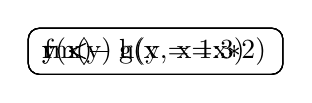
\begin{tikzpicture}
\cell{a}{\code{f(x)}}
\cell{b}{\code{y <- g(x = 1:3)}}
\cell{c}{\code{y <- h(y, x=x*2)}}
\cell{d}{\code{rm(y)}}
\end{tikzpicture}
\end{figure}
\gdef\AfterCells{}
\gdef\SatexReachedEnd{}
\end{document}
